\chapter{Implementation\label{cha:chapter5}}
This chapter deals with the implementation of the design presented in chapter \ref{cha:chapter4}. It was and is not the purpose of this work to implement a market-ready product. The focus is clearly on the conceptual part. To demonstrate the general realization of the proposed design, the implementation is done therefore only in the form of a prototype.


%\section{Development Environment\label{sec:impl_ecl}}	

\section{Tools \& Technologies\label{sec:impl_tools_tech}}	
This section gives an overview on the tools and technologies that have been used to simplify the implementation. The programming languages, which have been used to implement the framework, are Java and Python.

\subsection{Tools\label{sec:impl_tools}}
The following tools have been used to simplify, organize and test the implementation.

\paragraph{Eclipse Juno 4.2 IDE:\label{sec:impl_eclipse}} Eclipse is one of the widely used IDE for Java. It makes it easier to develop Java applications. 

\paragraph{Maven 3:\label{sec:impl_maven}} Maven is an open source build automation tool developed by the Apache Software Foundation. It uses an \ac{XML} file called \textit{pom.xml} to describe the software project being built, its dependencies, the build order, directories, and required plug-ins. It comes with predefined targets for performing certain well-defined tasks such as compilation of code, its packaging and how and where to deploy the project.


\paragraph{Advanced REST client:\label{sec:impl_advanced_rest_cl}} Advanced \ac{REST} client is a plugin within the Chrome browser and can help developers to create and test custom \ac{HTTP} requests. It has been used mainly to test the different \ac{REST} API, which have been developed within the framework.

\subsection{Technologies\label{sec:impl_technologies}}
In order to not reinvent the wheel again, most of the components in the framework are based on existing open source technologies. 

\paragraph{Spring Framework 3.1.1:\label{sec:impl_spring}} As described in \ref{sec:back_sp_fr}, the Spring framework is a lightweight solution and a very good base for building enterprise-ready applications. It provides an incredibly powerful and flexible collection of technologies and projects to improve enterprise Java application development. The following are some projects from the Spring framework, which have been used in developing the framework.

\subparagraph{Spring Security 3.1.1:\label{sec:impl_spring_sec}} Spring Security is a powerful and highly customizable authentication and access-control framework. It is the de-facto standard for securing Spring-based applications.

\subparagraph{Spring Data MongoDB 1.1.0:\label{sec:impl_spring_data}} Spring Data for MongoDB is part of the umbrella Spring Data project which aims to provide a familiar and consistent Spring-based programming model for for new datastores while retaining store-specific features and capabilities. The Spring Data MongoDB project provides integration with the MongoDB document database.

\subparagraph{Spring AMQP 1.1.3:\label{sec:impl_spring_amqp}} The Spring AMQP project applies core Spring concepts to the development of AMQP-based messaging solutions. It provide a "template" as a high-level abstraction for sending and receiving messages.

\paragraph{MongoDB 2.2.3:\label{sec:impl_mongo}} As described in \ref{sec:back_mongo}, MongoDB is a free and open-source document-oriented database and is completely schema-free and manages \ac{JSON}-style documents.

\paragraph{Elasticsearch 0.20.4:} Elasticsearch is an open-source, distributed, RESTful, search engine built on top of Apache Lucene.Its data model roots lie with schema-free and document-oriented databases, and as shown by the NoSQL movement, this model proves very effective for building applications.

\paragraph{RabbitMQ 3.0.1:} RabbitMQ is an open-source message broker, which implements the AMQP standard. It provides  robust messaging services for applications and is reliable and highly scalable.

\paragraph{NginX 1.2.6:} Nginx- engine-x pronounced - is a free, open-source, high-performance \ac{HTTP} server. Unlike traditional servers, Nginx does not rely on threads to handle requests. Instead it uses a much more scalable event-driven (asynchronous) architecture. This architecture uses small, but more importantly, predictable amounts of memory under load.

\paragraph{FFmpeg 0.9.2:} FFmpeg is the leading multimedia framework, able to decode, encode, transcode, mux, demux, stream, filter and play pretty much anything that humans and machines have created. It is an open source project licensed under LGPL version 2.1.

\paragraph{Tomcat 7.0.37:} Apache Tomcat is an open source software implementation of the Java Servlet and JavaServer Pages technologies. It powers numerous large-scale, mission-critical web applications across a diverse range of industries and organizations.

%%\pagebreak
%%\pagebreak

%\section{Used Open Source Tools\label{sec:impl_used_op_sr}}
\section{Framework Components\label{sec:impl_used_op_sr}}
This section describes how each component in the framework got implemented and realized.

\subsection{App Managment\label{sec:impl_app_man}}
The app management component is developed completely in Java and it is based on the Spring framework. Figure \ref{fig:eclipse_project} shows the project structure of this component withing the Eclipse IDE.

As shown in figure \ref{fig:eclipse_project}, the project consist of three java packages, namely \textit{de.fhg.fokus.ngni.cccd.model}, \textit{de.fhg.fokus.ngni.cccd.rest} and \textit{de.fhg.fokus.ngni.cccd.services}, and also four configurations file, which are, the maven configuration file \textit{pom.xml}, the \textit{web.xml} file, the logging configuration file \textit{log4j.xml} and the Spring configuration file \textit{cccd-config.xml}.

\begin{figure}[htb]
  \centering
  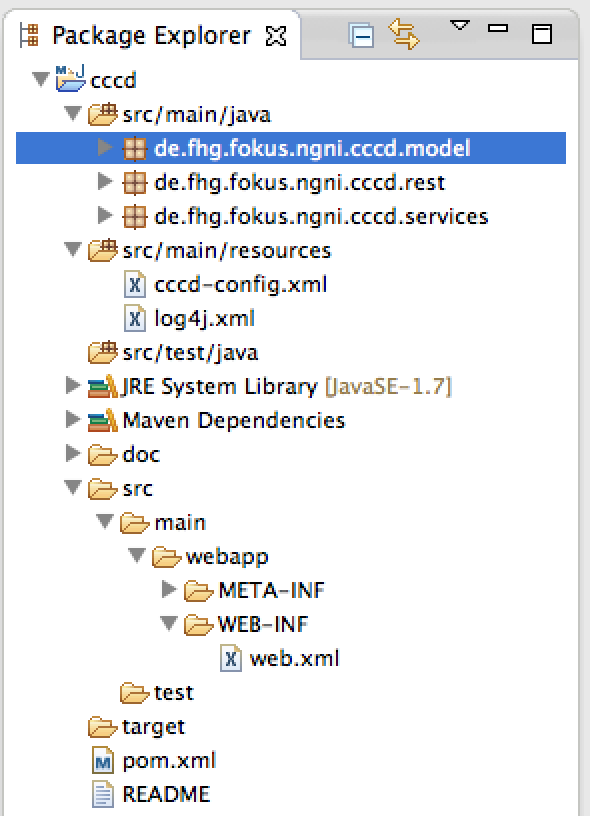
\includegraphics[scale=0.6]{eclipse_project.png}\\
  \caption{Eclipse Project Structure}
  \label{fig:eclipse_project}
\end{figure}

\pagebreak

The maven configuration file \textit{pom.xml} contains information about the project and configuration details used by Maven to build the project and also manages the dependencies which are needed for building the project.

Within the \textit{web.xml} file, one can set how to map a specific \ac{URL} to a particular servlet and Spring provides this in the form as in listing \ref{lst:web_xml}.

\begin{code}
\begin{minted}[frame=single,tabsize=2]{xml}
<web-app>
	<servlet>
		<servlet-name>cccd</servlet-name>
		<servlet-class>
			org.springframework.web.servlet.DispatcherServlet
		</servlet-class>
		<init-param>
			<param-name>
				contextConfigLocation
			</param-name>
			<param-value></param-value>
		</init-param>
		<load-on-startup>1</load-on-startup>
	</servlet>

	<servlet-mapping>
		<servlet-name>cccd</servlet-name>
		<url-pattern>/</url-pattern>
	</servlet-mapping>
</web-app>
\end{minted}
\caption{Excerpt from the web.xml configuration file}
\label{lst:web_xml}
\end{code}

In the above example at the servlet-mapping tag, this says that all URL("/") being requests should be handled by the \textit{cccd} servlet.  And what is the \textit{cccd} servlet and where to find it is declared in the servlet tag which tells Tomcat which Java class it should resolve this \textit{cccd} servlet to. Normally in none Spring applications one could just directly specify a class which inherits from the HttpServlet class. In Spring, however, this is where it actually enter the Spring Framework.  Instead of defining the class, which needs to be executed for this servlet directly, one need to specify only the class \textit{org.springframework.web.servlet.DispatcherServlet}. From this point onwards, the request and response are known by the Spring framework, so that one can apply Spring pre-processing and post-processing with special Spring modules, i.e. Security, Aspect Oriented Programming and so on.

The Spring configuration file \textit{cccd-config.xml} contains all of the Spring Web MVC-specific components (beans). In order to let the Spring framework detects all \textit{@Controller} beans, which provide all \ac{REST} interfaces, one need to set the tag \textit{context:component-scan} as follow:
\begin{code}
\begin{minted}[frame=single,tabsize=2]{xml}
<context:component-scan base-package="de.fhg.fokus.ngni.cccd.rest" />
\end{minted}
\end{code}

\paragraph{User Management:} For securing all \ac{REST} interfaces, the Spring Security project is used. Listing \ref{lst:cccd_security} is an excerpt from the configuration file \textit{cccd-config.xml} shows how to secure specific URI's with a specific role.
\begin{code}
\begin{minted}[frame=single,tabsize=2]{xml}
<sec:http create-session="stateless">
 	<sec:intercept-url pattern="/app/**" access="ROLE_USER" />
	<sec:intercept-url pattern="/users/**" access="ROLE_ADMIN" />
	<sec:http-basic />
</sec:http>
\end{minted}
\caption{Excerpt from the security part of the cccd-config.xml configuration file}
\label{lst:cccd_security}
\end{code}

The parameter \textit{create-session="stateless"} in listing \ref{lst:cccd_security} forces re-authentication with each request, in order to make it easier for load balancer as then request can go to any server machine, making location of server machine completely transparent and this leads to better scalability. The authentication mechanism is set through the tag \textit{sec:http-basic} in listing \ref{lst:cccd_security} and it enables the \ac{HTTP} Basic Auth, which should be used over \ac{HTTPS} of course, as it do not require a particularly complex negotiation.

By default in Spring, the user information are added to the application context file but in order to provide a more scalable source of user information, another authentication provider is implemented. This authentication provider is implemented in the class \textit{de.fhg.fokus.ngni.cccd.services.CustomUserDetailsService}, which implements the class  \textit{org.springframework.security.core.userdetails.UserDetailsService}. To configure the framework to use the implemented authentication provider, listing \ref{lst:cccd_auth} shows how it should be set withing the configuration file \textit{cccd-config.xml}.

\begin{code}
\begin{minted}[frame=single,tabsize=2,fontsize=\footnotesize]{xml}
<bean id="customUserDetailsService" 
	class="de.fhg.fokus.ngni.cccd.services.CustomUserDetailsService" />

<bean id="saltSource" 
	class="org.springframework.security.authentication.dao.ReflectionSaltSource">
	<property name="userPropertyToUse" value="username"/>
</bean>

<bean id="passwordEncoder" 
	class="org.springframework.security.authentication.encoding.Md5PasswordEncoder" />

<sec:authentication-manager  alias="authenticationManager" 
	erase-credentials="false">
	<sec:authentication-provider 
		user-service-ref="customUserDetailsService">
 		<sec:password-encoder ref="passwordEncoder">
 			<sec:salt-source ref="saltSource" />
 		</sec:password-encoder>
 	</sec:authentication-provider>
 </sec:authentication-manager>
\end{minted}
\caption{Configuring the authentication-provider within the cccd-config.xml configuration file}
\label{lst:cccd_auth}
\end{code}

The class \textit{CustomUserDetailsService} saves the user information in the repository. Thereby it does not save the password of the user as it is in a plain format within the repository, rather it merges the password first with a salt, which is the username here, see the tag \textit{<sec:password-encoder ref="passwordEncoder">} in listing \ref{lst:cccd_auth}, and then encodes it with an MD5 algorithm, which is provided through the class\textit{org.springframework.security.authentication.encoding.Md5PasswordEncoder}.

Where to save the user information exactly within the repository it is shown in the following excerpt from the configuration file \textit{cccd-config.xml}.
\begin{code}
\begin{minted}[frame=single,tabsize=2,fontsize=\footnotesize]{xml}
<bean id="mongoTemplate" class="org.springframework.data.mongodb.core.MongoTemplate">
	<constructor-arg ref="mongoDb" />
	<constructor-arg name="databaseName" value="users"/>
</bean>
\end{minted}
\end{code}

\paragraph{REST Interfaces:} All \ac{REST} interfaces are extending the class \textit{BaseCtrl.java}, which contains the Java driver instances for some components used in the \ac{REST} interfaces, like the repository, the search engine and the message broker, see listing \ref{lst:drivers_baseCtrl}, which is an excerpt from the class \textit{BaseCtrl.java}. The \textit{@Autowired} annotation will tell Spring to search within the configuration file \textit{cccd-config.xml} for a Spring bean which implements the required interface and place it automatically into the specified object, see listing \ref{lst:inj_baseCtrl}. How those Java driver instances are configured is shown in the next subsections.
\begin{code}
\begin{minted}[frame=single,tabsize=2,fontsize=\footnotesize]{java}
	/* MongoDB Java Driver */
	@Autowired
	protected Mongo mongoDb;
	
	/* Elasticsearch Java Driver */
	@Autowired
	Client esClient;
	
	/* RabbitMQ Java Driver */
	@Autowired
	protected RabbitTemplate amqpTemplate;
\end{minted}
\caption{Java driver Instances within BaseCtrl.java}
\label{lst:drivers_baseCtrl}
\end{code}

\begin{code}
\begin{minted}[frame=single,tabsize=2,fontsize=\footnotesize]{xml}
	<bean id="baseCtrl" class="de.fhg.fokus.ngni.cccd.rest.BaseCtrl">
	   	<property name="mongoDb" ref="mongoDb"/>
	   	<property name="esClient" ref="esClient"/>
	   	<property name="debugResponse" ref="debugResponse"/>
	   	<property name="customUserDetailsService" ref="customUserDetailsService"/>
	   	<property name="amqpTemplate" ref="amqpTemplate"/>
	</bean>
\end{minted}
\caption{Properties Injection of Class BaseCtrl.java}
\label{lst:inj_baseCtrl}
\end{code}

The class \textit{BaseCtrl.java} also contains two methods, namely \textit{canRead} and \textit{canWrite}. These methods provide the second level of the user management described in subsection \ref{sec:des_user_man}.

\subsection{Repository/Media Store\label{sec:impl_repo}}

The open source solution MongoDB is used as a repository within the framework. The specification GridFS, which is implemented in almost each MongoDB driver, is for storing and retrieving files within MongoDB. The GridFS is used as a media store for the framework.

How to configure the framework for using MongoDB is shown in listing \ref{lst:mongdb_driver}. Thereby a replication set of three MongoDB nodes are configured. 

\begin{code}
\begin{minted}[frame=single,tabsize=2,fontsize=\footnotesize]{xml}
    <bean id="mongoDb" class="com.mongodb.Mongo">
        <constructor-arg index="0">
            <list value-type="com.mongodb.ServerAddress">
                <bean class="com.mongodb.ServerAddress">
                    <constructor-arg index="0" value="10.0.0.73"/>
                    <constructor-arg index="1" value="27017"/>
                </bean>
                <bean class="com.mongodb.ServerAddress">
                    <constructor-arg index="0" value="10.0.0.74"/>
                    <constructor-arg index="1" value="27017"/>
                </bean>
                <bean class="com.mongodb.ServerAddress">
                    <constructor-arg index="0" value="10.0.0.75"/>
                    <constructor-arg index="1" value="27017"/>
                </bean>
            </list>
        </constructor-arg>
    </bean>
\end{minted}
\caption{Configuring the Java driver of MongoDB}
\label{lst:mongdb_driver}
\end{code}

By default the read and writes operations are done in the primary node but in order to enable read operations from secondary nodes, within the method \textit{setMongoDb} in Java class \textit{BaseCtrl.java} this following method is called. \textit{}
\begin{code}
\begin{minted}[frame=single,tabsize=2,fontsize=\footnotesize]{java}
	mongoDb.setReadPreference(ReadPreference.secondaryPreferred());
\end{minted}
\end{code}

The installation and configuration of MongoDB on Ubuntu is described in section \ref{sec:eval_te_en_mongo}.

\subsection{Search Engine\label{sec:impl_se_en}}
As an open source solution for the search engine, the Elasticsearch project is used. Listing \ref{lst:elasticsearch_driver} shows how to configure the Java driver in the configuration file \textit{cccd-config.xml}.

\begin{code}
\begin{minted}[frame=single,tabsize=2,fontsize=\footnotesize]{xml}
	<bean id="esClient" class="org.elasticsearch.client.transport.TransportClient" />
	
	<bean class="org.springframework.beans.factory.config.MethodInvokingFactoryBean">
		<property name="targetObject"><ref local="esClient"/></property>
		<property name="targetMethod"><value>addTransportAddresses</value></property>
		<property name="arguments"> 
			<list value-type="org.elasticsearch.common.transport.InetSocketTransportAddress">
				<bean class="org.elasticsearch.common.transport.InetSocketTransportAddress">
					<constructor-arg index="0" value="10.0.0.186"/>
					<constructor-arg index="1" value="9300"/>
				</bean>
		 	</list>
		</property>
	</bean>
\end{minted}
\caption{Configuring the Java driver of Elasticsearch}
\label{lst:elasticsearch_driver}
\end{code}

The installation and configuration of Elasticsearch on Ubuntu is described in section \ref{sec:eval_te_se}.

\subsection{Message Broker\label{sec:impl_mb}}
The open source project RabittMQ is used as a message broker. Listing \ref{st:rabbitmq_driver}  shows how to configure the framework for using RabittMQ as a message broker. The default username/password for RabbitMQ are \textit{guest}/\textit{guest}.

\begin{code}
\begin{minted}[frame=single,tabsize=2,fontsize=\footnotesize]{xml}
	<bean id="connectionFactory" class="org.springframework.amqp.rabbit.connection.CachingConnectionFactory">
	    <constructor-arg value="10.0.0.140" />
		<property name="username" value="guest" />
	    <property name="password" value="guest"/>
	</bean>
	
	<rabbit:template id="amqpTemplate" connection-factory="connectionFactory"/>
\end{minted}
\caption{Configuring the Java driver of RabbitMQ}
\label{lst:rabbitmq_driver}
\end{code}

The installation and configuration of RabittMQ on Ubuntu is described in section \ref{sec:eval_te_en_rabittmq}.

\subsection{Content Adaptation\label{sec:des_ar_ov}}
As shown in figure \ref{fig:content_adaptation_overview} in the design chapter, the content adaptation components consists internally of two components, namely the media encoder and the media segmenter. 

For the media encoder, the open source project FFmpeg is used. 

As a media segmenter, this open source media segmenter/distributor \cite{hlvssad} is used. This project makes it easier to set up a live streaming server using Apple's \ac{HTTP} streaming protocol. The project includes ruby scripts and a C program that use FFMpeg to encode and segment an input video stream in the correct format for use with the \ac{HTTP} streaming protocol.

For consuming messages from the message broker and process them, the python script cccdCA.py is implemented. This script is started automatically with Linux and listens for new messages from a queue called \textit{newMMfiles} within the message broker. %The message format is shown in listing \ref{}. 

After receiving a message from the message broker, which contain the \textit{ObjectId} of the video file and the app name \textit{appName}, the python script downloads the video file which needs to be processed from the GridFS media store to the \textit{/tmp/} directory. The file is then passed to the media segmenter/distributor a long with the directory name within the content distribution component where to upload the output files to. This directory name is basically build from \textit{appName/ObjectId}. The segmenter/distributor uploads the output files via FTP, which needs to be already configured on the content distribution component. If the message is successfully processed, the python script updates the metadata of the video file in the repository and adds a new tag which points to the index file of the transcoded/scaled video.

The installation and configuration of this component on Ubuntu is described in section \ref{sec:eval_te_ca}.
%The python script process the message in the following order:
%\begin{itemize}
%\item extract the \textit{ObjectId}, \textit{appName} keys from the message
%\item download the file with the same \textit{ObjectId} from GridFS(media store) and rename it to value of \textit{ObjectId} and then save it in \textit{/tmp/} directory
%\item update the configuration 
%\end{itemize}
	
\subsection{Content Distribution\label{sec:impl_cdn}}
The content distribution component consists internally of two components, which are a python script called \textit{cccdCD.py} and the open source project NginX as a \ac{HTTP} server.

In order to secure the video file link within the content distribution component, the \textit{HttpSecureLinkModule} from NginX is used. This module is not compiled by default and must be enabled while compiling the source code of NginX.

For consuming messages from the message broker and process them, the python script \textit{cccdCD.py} is implemented. This script is started automatically with Linux and listens for new messages from either a queue called \textit{AppEvents} or a queue called \textit{DocDelete} within the message broker. %A message notification will be sent to the queue \textit{AppEvents} either by  creating or deleting apps so that there respective directorys within the content distribution component can be created or deleted. Another message notification will be sent to the queue \textit{DocDelete} by deleting a document from an app so that its related contents within the content distribution component can be deleted.
%The message format is shown in listing \ref{} and listing \ref{} respectively.

Listing \ref{lst:cccdCD} shows a method from the script \textit{cccdCD.py} which process a message coming from the queue \textit{AppEvents}. The message can be either a notification of a new created app(\textit{status==created}) or a notification of a deleted app(\textit{status==deleted}). In case of a creation of a new app the python script creates a configuration file for the NginX server and also creates a directory with the same name as the \textit{appName} within the WWW directory of the NginX server. In case of a deletion of an app, the python script deletes the app directory along with its contents.
\pagebreak

\begin{code}
\begin{minted}[frame=single,tabsize=2,fontsize=\footnotesize]{python}
jsonBody = json.loads(body)
if(jsonBody['status']=="created"):
	file = open(locations_dir+jsonBody['appName']+'.conf', 'w+')
	file.write(str(location_tmpl.safe_substitute(dict(app=jsonBody['appName']
		,secret=jsonBody['secret']))))
	file.close()
	if not os.path.exists(www_dir+jsonBody['appName']):
		os.makedirs(www_dir+jsonBody['appName'])
		#reload the nginx server
		os.system("%s %s %s"%(nginx_bin, '-s', 'reload'))
	if(jsonBody['status']=="deleted"):
		os.remove(locations_dir+jsonBody['appName']+'.conf')
		shutil.rmtree(www_dir+jsonBody['appName'], 
			ignore_errors=False, onerror=handleRemoveReadonly)
		#reload the nginx server
		os.system("%s %s %s"%(nginx_bin, '-s', 'reload'))
\end{minted}
\caption{cccdCD.py python script}
\label{lst:cccdCD}
\end{code}

Another message notification will be sent to the queue \textit{DocDelete} by deleting a document from an app so that its related contents within the content distribution component can be deleted.

Listing \ref{lst:locations_nginx} shows an example of a created configuration file for a new app called \textit{app1} with \textit{pass123} as a secret word. From now on each request to the URI \textit{/app1/} must have the MD5 hash as a parmeter, which is built from the secret word, the URI(the path of the requested file) and the expiration time. How this MD5 hash calculated is shown on the documentation site of NginX \cite{nginx:securelink}.

\begin{code}
\begin{minted}[frame=single,tabsize=2,fontsize=\footnotesize]{php}
location /app1/ {
        secure_link $arg_st,$arg_e;
        secure_link_md5 pass123$uri$arg_e;
        if ($secure_link = "") {
                return 403;
        }
        if ($secure_link = "0") {
                return 403;
        }
}
\end{minted}
\caption{Sample configuration file for locations within NginX}
\label{lst:locations_nginx}
\end{code}


%\subsubsection{HTTP-Live-Video-Stream-Segmenter-and-Distributor\label{sec:impl_http_li}}
%	\subsubsection{NginX\label{sec:impl_ngi}}
	
	
%	\subsubsection{RabbitMQ\label{sec:impl_ra_mq}}
	
%	\subsection{User API\label{sec:des_api}}
%	\subsubsection{SPRING DATA - REST\label{sec:des_api}}

%\section{Components Integration and Configuration\label{sec:impl_comp_in}}

%\section{REST API\label{sec:impl_rest_api}}